
\chapter{The Cut-Matching Game: Expanders via Max Flow}

In this chapter, we learn about a new algorithm to compute expanders that employs max flow as a subroutine.

\section{Introduction}

We start with a review of expanders where make a subtle change the notion of an expander in comparison to chapter \ref{chap:cheegersInequality} to ease the exposition.

\paragraph{Definitions.} We let $G=(V,E)$ be an unweighted, connected graph in this chapter, and let $\dd$ be the degree vector, $E(S,V \setminus S)$ denote the set of edges crossing the cut $A,B$

Given set $\emptyset \subset S \subset V$, then we define the \textbf{sparsity} $\psi(S)$ of $S$ by
\[
\psi(S) = \frac{|E(S, V \setminus S)|}{ \min\{|S|, |V \setminus S| \} } 
\]
Note that \textbf{sparsity} $\psi(S)$ differs from \textbf{conductance} $\phi(S) = \frac{|E(S, V \setminus S)|}{ \min\{\vol(S), \vol(V \setminus S) \} }$, as defined in \ref{chap:cheegersInequality}, in the denominator. It is straight-forward to see that in a connected graph $\psi(S) \geq \phi(S)$ for all $S$. 

Clearly, we again have $\psi(S) = \psi(V \setminus S)$. We define the \emph{sparsity} of a graph $G$ by $\psi(G) = \min_{\emptyset \subset S \subset V} \psi(S)$. For any $\psi \in (0, n]$, we say a graph $G$ is a $\psi$-expander with regard to sparsity, if $\psi(G) \geq \psi$. When the context is clear, we simply say that $G$ is a $\psi$-expander. 

\paragraph{The Main Result.} The main result of this chapter is the following theorem.

\begin{theorem}
There is an algorithm $\textsc{SparsityCertifyOrCut}(G, \psi)$ that given a graph $G$ and a parameter $0 <\psi \leq 1$ either: 
\begin{itemize}
    \item \emph{Certifies} that $G$ is a $\Omega(\psi/\log^2 n)$-expander with regard to sparsity, or
    \item Presents a \emph{cut} $S$ such that $\psi(S) \leq O(\psi)$.
\end{itemize}
The algorithm runs in time $O(\log^2 n) \cdot (T_{max\_flow}(G) + m)$ where $T_{max\_flow}(G)$ is the time it takes to solve a Max Flow problem on $G$\footnote{Technically, we will solve problems with two additional vertices and $n$ additional edges but this will not change the run-time of any known max-flow algorithm asymptotically.}.
\end{theorem}

We will see in the homework for this week that the above guarantees can also be given if we are looking for an expander with regard to conductance. Using current state-of-the art Max Flow results, the above problem can be solved in $\tilde{O}(m + n^{4/3+o(1)})$ time. 

\section{Embedding Graphs into Expanders}

Let us start by exploring the first key idea behind the algorithm. We therefore need a definition of what it means to embed one graph into another.

\paragraph{Definition of Embedding.} Given graphs $H$ and $G$ that are defined over the same vertex set, then we say that a function $\textsc{Embed}_{H \xrightarrow{} G}$ is an \emph{embedding} if it maps each edge $(u,v) \in H$ to a $u$-to-$v$ path $P_{u,v} = \textsc{Embed}_{H \xrightarrow{} G}(u,v)$ in $G$. 
\begin{figure}[!ht]
    \centering
    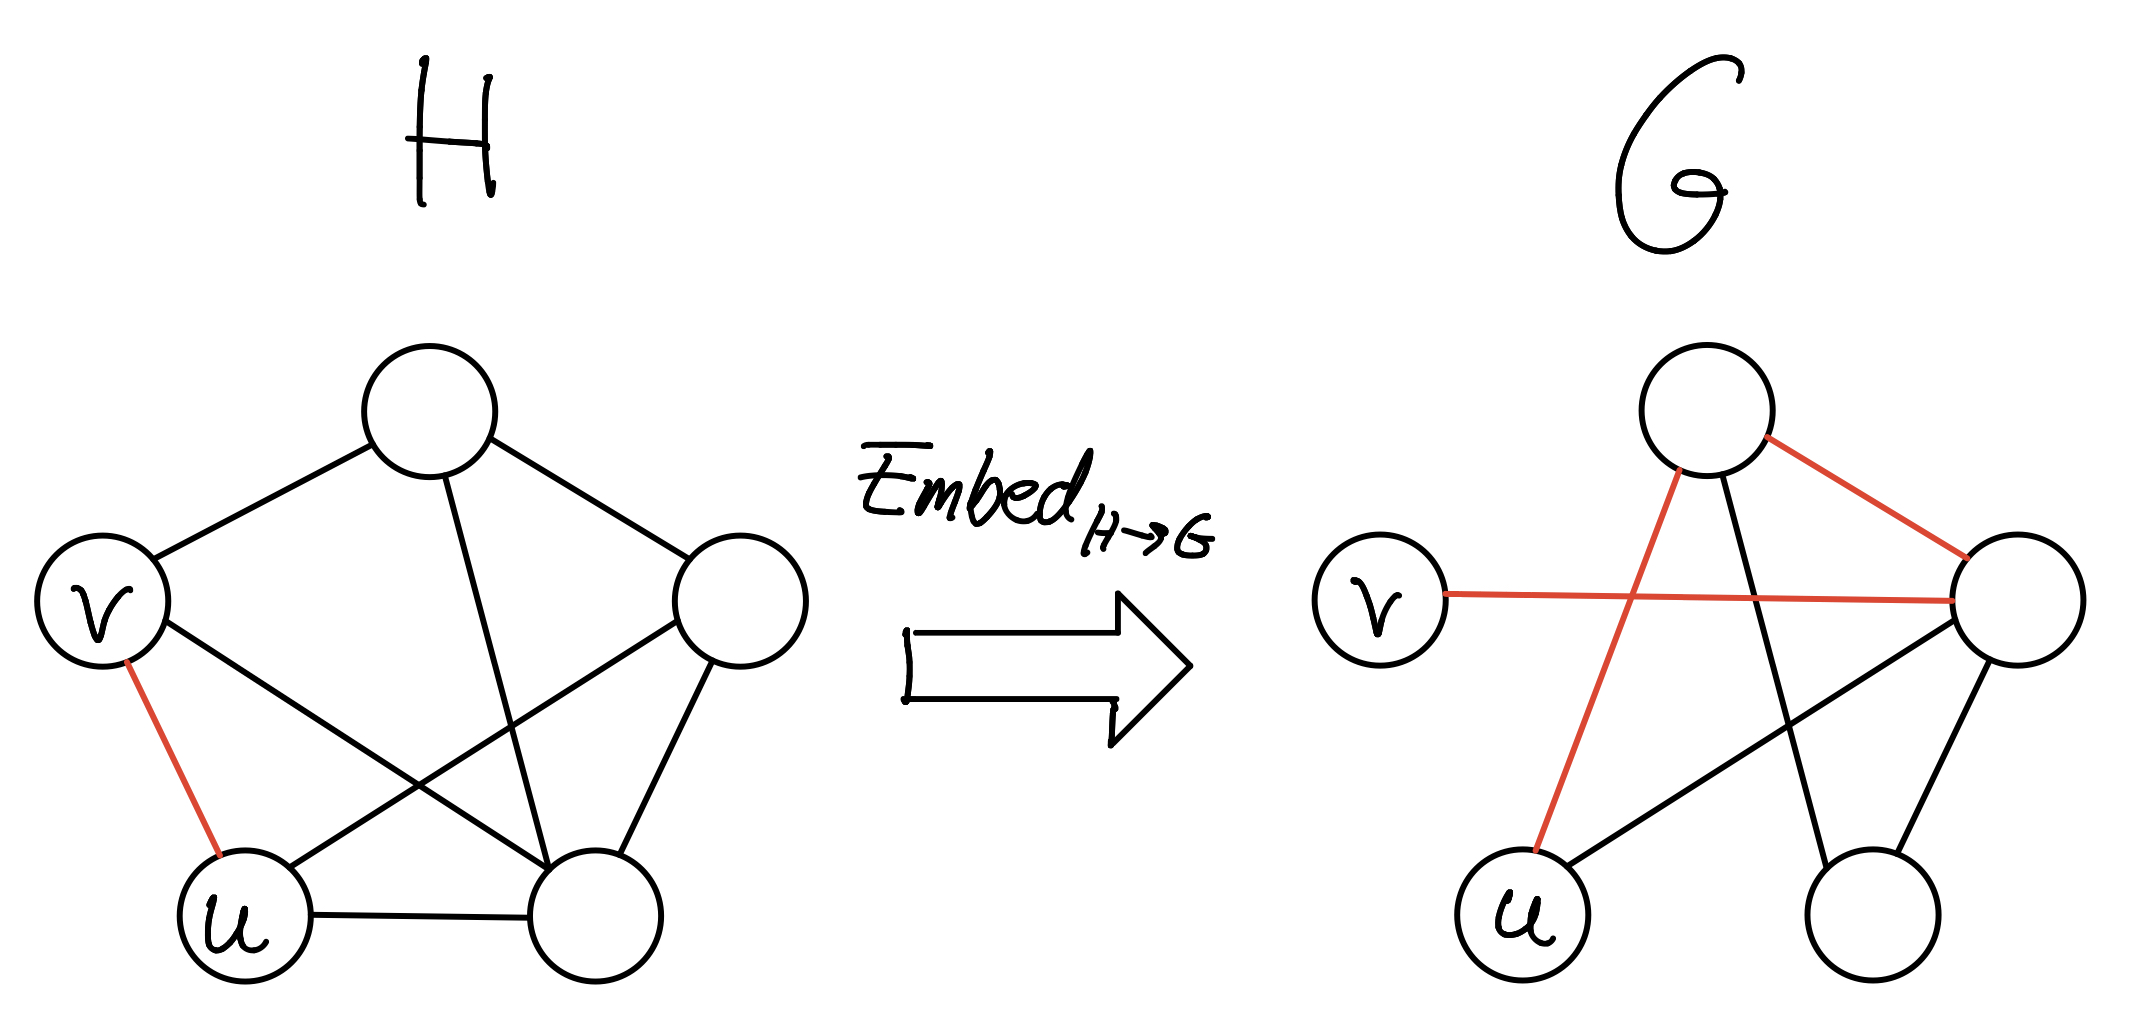
\includegraphics[scale=0.2]{./fig/embedGraph_lectureCutMatching.jpeg}
    \caption{In this example the red edge $(u,v)$ in $H$ is mapped to the red $u$-to-$v$ path in $G$.}
    \label{fig:my_label}
\end{figure}

We say that the \emph{congestion} of $\textsc{Embed}_{H \xrightarrow{} G}$ is the maximum number of times that any edge $e \in E(G)$ appears on any embedding path: \[
\congestion(\textsc{Embed}_{H \xrightarrow{} G}) = \max_{e \in E(G)} |\{ e' \in E(H) \;|\; e \in \textsc{Embed}_{H \xrightarrow{} G}(e') \}|.
\]

\paragraph{Certifying Expander Graphs via Embeddings.} Let us next prove the following lemma that is often consider Folklore.

\begin{lemma}\label{lma:folklore_embedding}
Given a $\frac{1}{2}$-expander graph $H$ and an embedding of $H$ into $G$ with congestion $C$, then $G$ must be an $\Omega\left(\frac{1}{C}\right)$-expander. 
\end{lemma}
\begin{proof}
Consider any cut $(S, V \setminus S)$ with $|S| \leq |V \setminus S|$. Since $H$ is a $\psi$-expander, we have that $|E_H(S, V \setminus S)| \geq |S|/2$. We also know by the embedding of $H$ into $G$, that for each edge $(u,v) \in E_H(S, V \setminus S)$, we can find path a $P_{u,v}$ in $G$ that also has to cross the cut $(S, V \setminus S)$ at least once. But since each edge in $G$ is on at most $C$ such paths, we can conclude that at least $|E_H(S, V \setminus S)|/ C \geq |S|/2C$ edges in $G$ cross the cut $(S, V \setminus S)$. 
\end{proof}
 
Unfortunately, the reverse of the above lemma is not true, i.e. even if there exists no embedding from $1/2$-expander $H$ into $G$ of congestion $C$, then $G$ might still be an $\Omega\left(\frac{1}{C}\right)$-expander. 

\section{The Cut-Matching Algorithm}

Although there are still some missing pieces, let us next discuss the algorithm   \ref{algo:cutMatchingGame}. The algorithm runs for $T$ iterations where we will later find that the right value to set $T$ to is in $\Theta(\log^2 n)$. 

\begin{algorithm}[H]
    \For{$i = 0,1,2, \dots, T$}{
        $(S_i, \overline{S}_i) \gets \textsc{FindBiPartition}(G, \{M_1, M_2, \dots, M_{i}\})$ \tcp*{Assume  $|S| = |\overline{S}| = n/2$}
        Solve the flow problem on $G$ where each vertex $e \in E$ receives capacity $\cc(e) = 1/\psi$ and the demand at each edge $v \in S$ is $+1$ and for each $v \in \overline{S}$ is $-1$, by introducing a super-source $s$ and super-sink $t$\;
        \If{flow procedure returns a flow $\ff$ with $\val(f) = n/2$}{
            Remove $s,t$ to derive $S$-$\overline{S}$ flow; then decompose flow $\ff$ into flow paths $P_1, P_2, \dots, P_{n/2}$\;
            Create a matching $M_{i}$ where for each $s$-to-$\overline{s}$ flow path $P_i$, we add $(s, \overline{s})$ to $M_i$.
        }\Else{
            \Return the minimum cut $(X_S, X_{\overline{S}})$ in the flow problem after removing the super-source $s$ and the super-sink $t$ from the two sets.
        }
    }
    \Return $H = \bigcup_{i} M_i$
  \caption{\textsc{SparsityCertifyOrCut}$(G, \psi)$}
  \label{algo:cutMatchingGame}
\end{algorithm}

\begin{figure}[!ht]
    \centering
    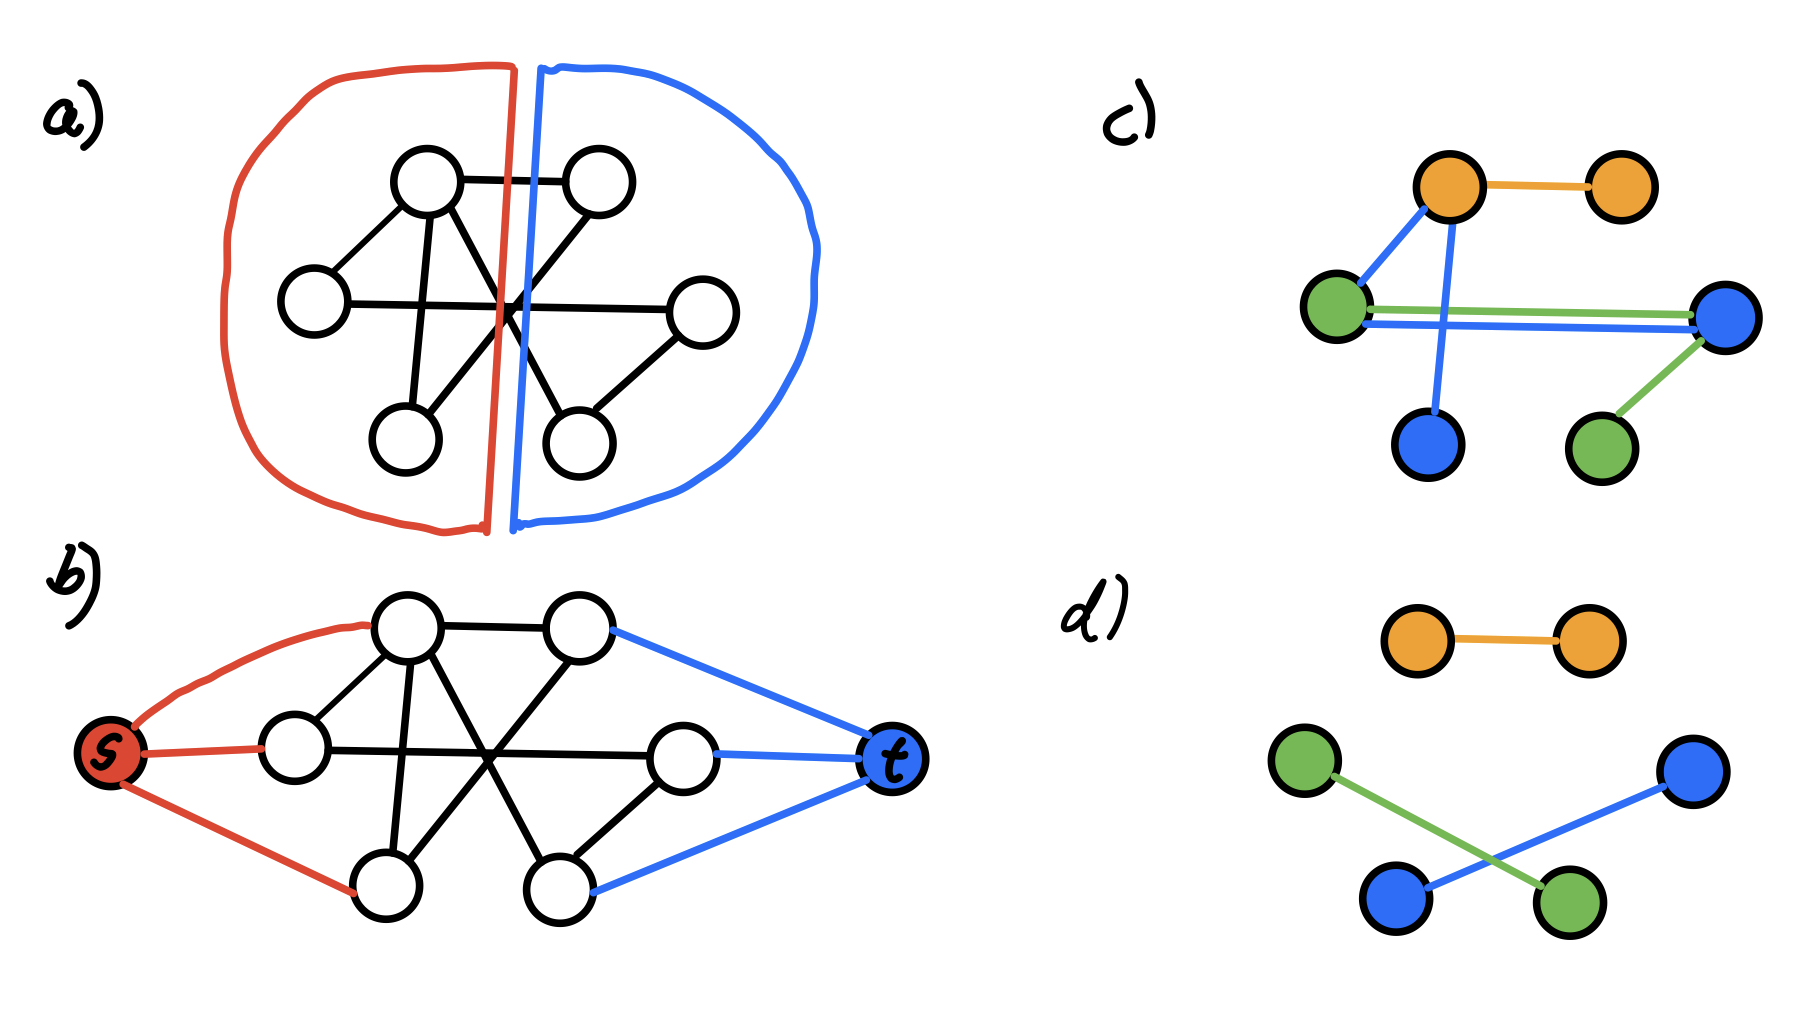
\includegraphics[scale=0.2]{./fig/AlgorithmProcessing_lectureCutMatching.jpeg}
    \caption{Illustration of the steps of the Algorithm. In a), a bi-partition of $V$ is found. In b), the bi-partition is used to obtain a flow problem where we inject one unit of flow to each vertex in $S$ via super-source $s$ and extract one unit via super-sink $t$. c) A path flow decomposition. For each path, the first vertex is in $S$ and the last vertex in $\overline{S}$. d) We find $M_i$ to be the one-to-one matching between endpoints in $S$ and $\overline{S}$ defined by the path flows.}
    \label{fig:my_label}
\end{figure}

\paragraph{Beginning of an Iteration.} In each iteration of the algorithm, we first invoke a sub-procedure $\textsc{FindBiPartition}(\cdot)$ that returns a cut $(S,\overline{S})$ (where $\overline{S} = V \setminus S$) that partitions the vertex set into two equal-sized sides. Here, we implicitly assume that the number of vertices $n$ is even which is w.l.o.g. 

Next, the algorithm creates a flow problem where each vertex $s \in S$ has to send exactly one unit of flow and each vertex $\overline{s} \in S$ has to receive exactly one unit of flow. We therefore introduce dummy nodes $s$ and $t$, add for each vertex $v \in S$ an edge of capacity $1$ between $s$ and $v$; and for each vertex $v \in \overline{S}$ and edge between $t$ and $v$ of capacity $1$. We set the capacity of edges in the original graph $G$ to $1/\psi$ (which we assume wlog to be integer).

\paragraph{The If Statement.} If the flow problem can be solved exactly, then we can find a path decomposition of the flow $\ff$ in $\tilde{O}(m)$ time (for example using a DFS) where each path starts in $S$ ends in $\overline{S}$ and carries one unit of flow\footnote{For simplicity, assume that the returned flow is integral.}. This defines a one-to-one correspondence between the vertices in $S$ and the vertices in $\overline{S}$. We capture this correspondences in the matching $M_i$. We will later prove the following lemma.

\begin{lemma}
If the algorithm returns after constructing $T$ matchings, for an appropriately chosen $T = \Theta(\log^2 n)$, then the graph $H$ returned by the algorithm is a $\frac{1}{2}$-expander and $G$ can be embedded into $H$ with congestion $O(\log^2 n/ \psi)$.
\end{lemma}

\paragraph{The Else Statement.} On the other hand, if the flow problem on $G$ could not be solved, then we return the min-cut of the flow problem. Such a cut can be found in $O(m)$ time by using the above reduction to an $s$-$t$ flow problem on which one can compute maximum flow $\ff$ from which the $s$-$t$ min-cut can be constructed by following the construction in the proof of \Cref{thm:maxFlowEqualsMinCut}.

It turns out that this min-cut already is a sparse cut by the way our flow problem is defined.

\begin{lemma}
If the algorithm finds a cut $(X_S, X_{\overline{S}})$, then the returned cut satisfies $|E_G(X_S \setminus \{s\}, X_{\overline{S}} \setminus \{t\})| = O(\psi)$.
\end{lemma}
\begin{proof}
First observe that since a min-cut was returned, we have that $|E_G(X_S, X_{\overline{S}})| < n/2$ (otherwise we could have routed the demands).

Let $n_s$ be the number of edges incident to the super-source $s$ that cross the cut $(X_S, X_{\overline{S}})$. Let $n_t$ be the number of edges incident to $t$ that cross the cut $(X_S, X_{\overline{S}})$.

\begin{figure}[!ht]
    \centering
    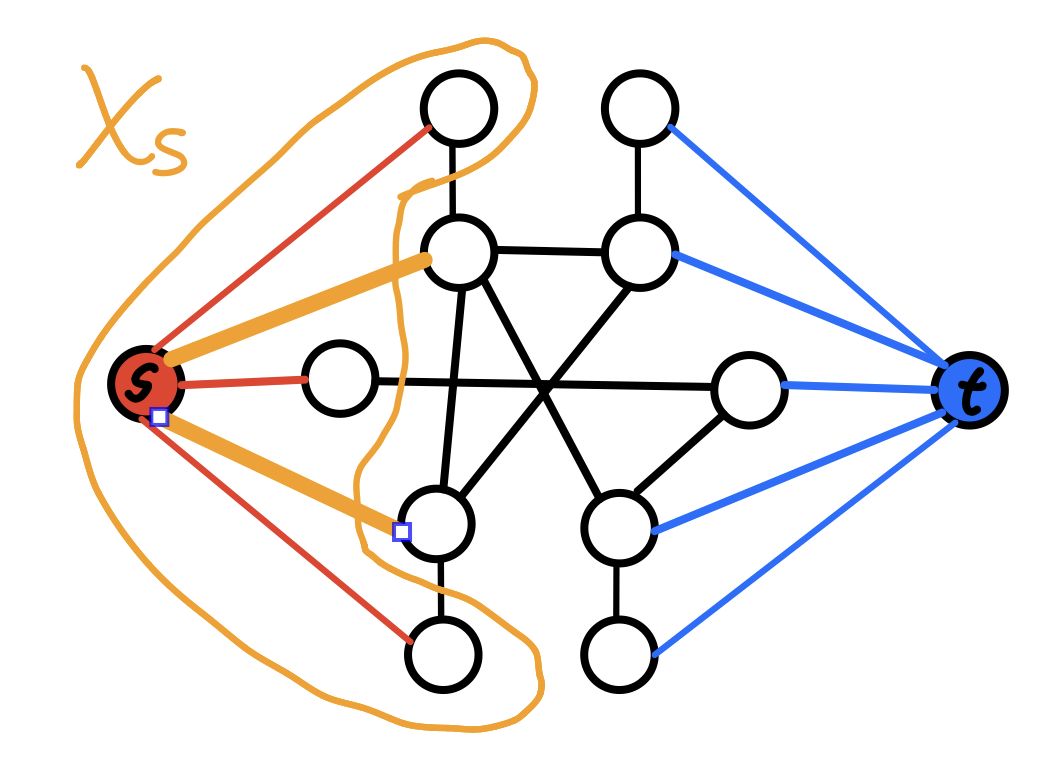
\includegraphics[scale=0.2]{./fig/FewEdgesCrossCut_lectureCutMatching.jpeg}
    \caption{Set $X_S$ is enclosed by the orange circle. The thick orange edges are in the cut and incident to super-source $s$. Thus they count towards $n_s$. Here $n_s = 2, n_t = 0$. Note that all remaining edges in the cut are black, i.e. were originally in $G$ and therefore have capacity $1/\psi$.}
    \label{fig:my_label}
\end{figure}

Observe that after taking away the vertices $s$ and $t$, the cut $(X_S \setminus \{s\}, X_{\overline{S}} \setminus \{t\})$ has less than $n/2 - n_s - n_t$ capacity. But each remaining edge has capacity $1/\psi$, so the total number of edges in the cut can be at most $\psi \cdot (n/2 - n_s - n_t)$. Since $X_S \setminus \{s\}$ is of size at least $n/2-n_s$, and $X_{\overline{S}} \setminus \{t\}$ is of size at least $n/2-n_t$, we have that the induced cut in $G$ has
\[
    \psi(X_S \setminus \{s\}) < \frac{\psi \cdot (n/2 - n_s - n_t)}{\min\{ n/2 - n_s, n/2 - n_t\}} \leq \psi.
\]
\end{proof}

\section{Constructing an Expander via Random Walks}

Next, we give the implementation and analysis for the procedure $\textsc{FindBiPartition}(\cdot)$. We start however by giving some more preliminaries.

\paragraph{Random Walk on Matchings.} Let $\{M_1, M_2, \dots, M_{T+1}\}$ be the set of matchings we compute (if we never find a cut). In the $i^{th}$-step of a $t$-step lazy random walk, a particle at a vertex $j$ stays put with probability $1/2$, and traverses the edge in matching $M_i$ incident to $j$ with probability $1/2$. 

We let $\pp_{j \mapsto i}^t$ denote the probability that a particle that started at vertex $j$ is at vertex $i$ after a $t$-step lazy random walk. We let $\pp_i^t = [\pp_{1 \mapsto i}^t\; \pp_{2 \mapsto i}^t\; \dots \;\pp_{n \mapsto i}^t]$. Note that for each edge $(i,j) \in M_t$, we have that 
\[
\pp_i^{(t+1)} = \frac{1}{2} \pp_i^t + \frac{1}{2} \pp_j^t = \pp_j^{(t+1)}.
\]
We define the projection matrix $\proj^t = [\pp_1^{t}, \pp_2^{t}, \dots, \pp_n^{t}]^\trp$ that maps an initial probability distribution $\dd$ to the probability distribution over the vertices that the random walk visits them at step $t$. You will prove in the exercises that $\proj^t$ is \emph{doubly-stochastic}.

We say that a lazy random walk is \emph{mixing} at step $t$, if for each $i,j$, $\pp_{j \mapsto i}^t \geq 1/(2n)$. 

\begin{lemma}
If $t$-step lazy random walk is \emph{mixing}, then $H = \bigcup_{i \leq t} M_i$ is a $\frac{1}{2}$-expander.
\end{lemma}
\begin{proof}
Consider any cut $(S, \overline{S})$ with $|S| \leq |\overline{S}|$. It is convenient to think about the random walks in terms of probability mass that is moved around. Observe that each vertex $j \in \overline{S}$ has to push at least $1/(2n)$ units of probability from $j$ to $i$ (by definition of mixing). 

\begin{figure}[!ht]
    \centering
    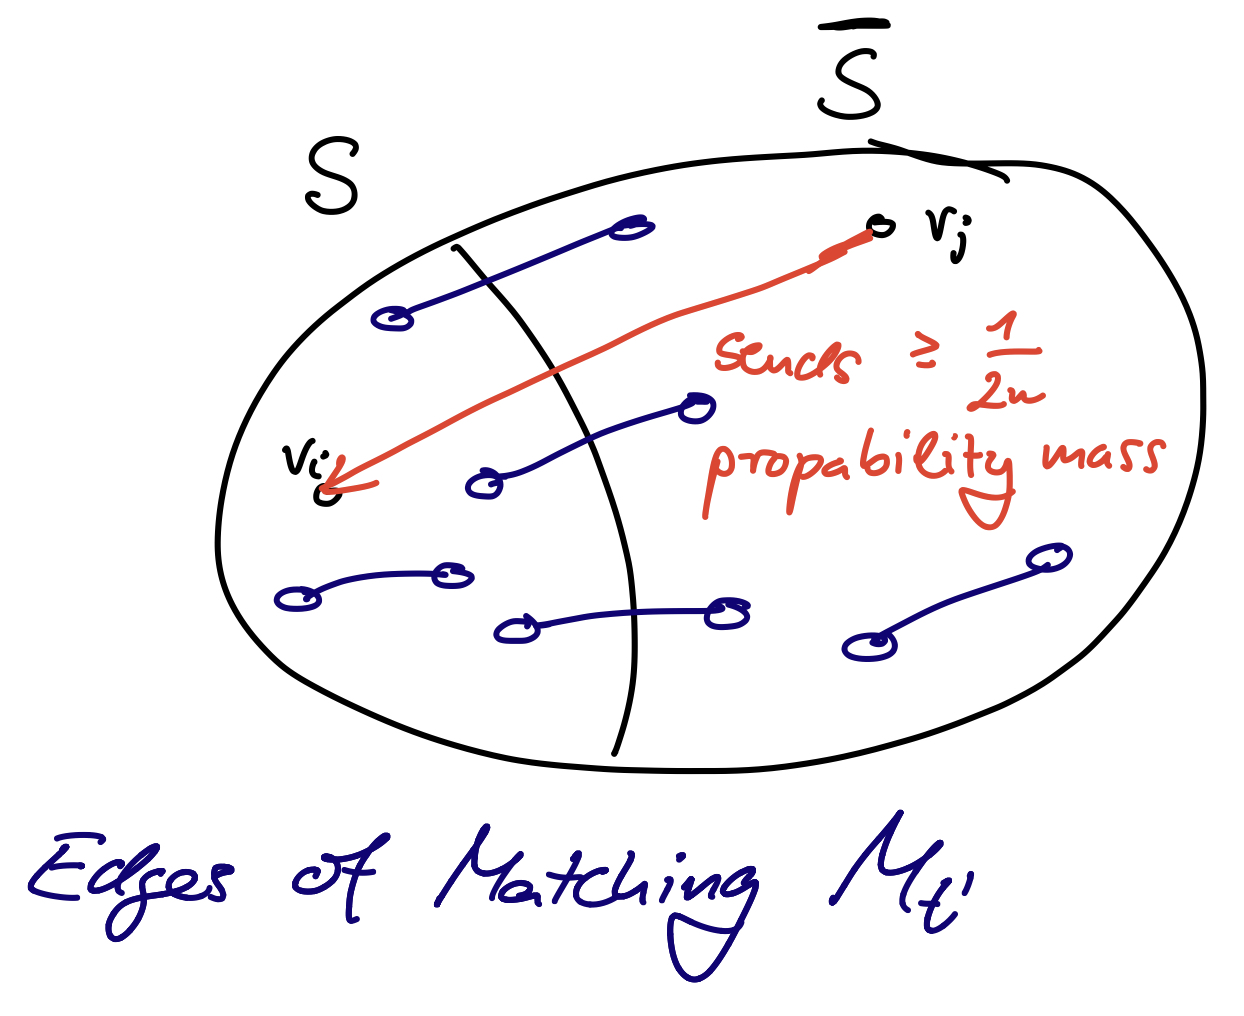
\includegraphics[scale=0.15]{./fig/MixingWalkIsExpander_lectureCutMatching.jpeg}
    \caption{Each vertex $j \in \overline{S}$ sends at least $1/(2n)$ probability mass to $i$ (red arrow). But in order to transport it, it does have to push the mass through edges in the matchings $M_1, M_2, \dots, M_t$ that cross the cut.}
    \label{fig:my_label}
\end{figure}

Clearly, to move the mass from $\overline{S}$ to $S$ it has to use the matching edges that also cross the cut.

Now observe that since there are $\geq n/2$ vertices in $\overline{S}$, and each of them has to push $\geq 1/(2n)$ mass to $i$, the total amount of probability mass pushed through the cut for $i$ is $\geq 1/2$. Since there are $|S|$ such vertices $i$, the total amount of mass that has to cross the cut is $\geq |S|/2$. 
But note, that after each step of the random walk, the total probability mass at each vertex is exactly $1$. Thus, at each step $t'$, each edge in $M_{t'}$ crossing the cut can push at most $1/2$ units of probability mass over the cut (and thereafter the edge is gone). 

It follows that there must be at least $|S|/2$ edges in the matchings $M_1, M_2, \dots M_{t}$. But this implies that $H = \cup_i M_i$ is a $\frac{1}{2}$-expander.

\end{proof}

\paragraph{Implementing $\textsc{FindBiPartition}(\cdot)$.} We can now give away the implementation of $\textsc{FindBiPartition}(\cdot)$ which you can find below.

\begin{algorithm}[H]
    Choose random $n$-dimensional vector $\rr$ orthogonal to $\vecone$.\;
    Compute vector $\uu = \proj^t \rr$, i.e. each $\uu_i = \pp_i^t \cdot \rr$\;
    Let $S$ be the $n/2$ smallest vertices w.r.t. $\uu$; and $\overline{S}$ be the $n/2$ largest w.r.t $\uu$ (ties broken arbitrarily but consistently).\;
    \Return $(S, \overline{S})$
  \caption{\textsc{FindBiPartition}$(G, \{M_1, M_2, \dots, M_t\})$}
  \label{algo:findBiPartition}
\end{algorithm}

The central claim, we want to prove is the following: given a potential function for the random walk at step $t$
\[
    \Phi^t = \sum_{i,j} (\pp_{j \mapsto i}^t - 1/n)^2 = \sum_{i} \|\pp_{i}^t - \vecone/n\|_2^2.
\]
\begin{claim}\label{clm:mainClaimCutMatching}
In the algorithm $\textsc{SparsityCertifyOrCut}(\cdot)$, we have $\mathbb{E}[\Phi^{t} - \Phi^{(t+1)}] \geq \Omega(1/\log n) \Phi^{t}$.
\end{claim}
\begin{corollary}
For appropriate $T = \Theta(\log^2 n)$, the algorithm $\textsc{SparsityCertifyOrCut}(\cdot)$ has $\Phi^{(T+1)} \leq 4/n^2$.
\end{corollary}

The corollary follows straight-forwardly since $O(\log n)$ iterations suffice with high probability to reduce the potential by factor $\frac{1}{2}$ (you can use Chernoff here). Then, after $O(\log n)$ such phases consisting of $O(\log n)$ iterations, the potential drops to $1/n^d$ for any $d$ which then goes into the constant factors.

We further observe that this implies that $\{M_1, M_2, \dots, M_{T+1}\}$ is mixing (you can straight-forwardly prove it by a proof of contradiction), and thereby we conclude the proof of our main theorem. 

Let us now give the prove of Claim \ref{clm:mainClaimCutMatching}: 

\paragraph{Interpreting the Potential Reduction.} Let us start by observing 
\begin{align*}
     \Phi^{t} - \Phi^{(t+1)} = \sum_{i} \|\pp_{i}^t -\vecone/n\|_2^2 + \sum_{i} \|\pp_{i}^{(t+1)} -\vecone/n\|_2^2
\end{align*}
Considering now \textbf{any} matching $M$, and an edge $(i,j) \in M$. We can re-write the former sum as $\sum_{i} \|\pp_{i}^t -\vecone/n\|_2^2 = \sum_{(i,j) \in M} \|\pp_{i}^t -\vecone/n\|_2^2 + \|\pp_{j}^t -\vecone/n\|_2^2$ and we can do the same for the $t+1$-step walk probabilities. Further, note that for $(i,j) \in M$, we have $\pp_i^{(t+1)} = \pp_j^{(t+1)} = \frac{\pp_i^t+ \pp_j^t}{2}$. Thus,
\begin{align*}
     \Phi^{t} - \Phi^{(t+1)} = \sum_{(i,j)}  \|\pp_{i}^t -\vecone/n\|_2^2 + \|\pp_{j}^t -\vecone/n\|_2^2 - 2 \left\|\frac{\pp_i^t+ \pp_j^t}{2}\right\|_2^2.
\end{align*}
Finally, we can use the formula $\|\xx\|^2 + \|\yy\|^2 - 2 \|(\xx + \yy)/2\|^2 = \frac{1}{2} \| \xx - \yy\|^2$ term-wise to derive 
\begin{align*}
     \Phi^{t} - \Phi^{(t+1)} = \frac{1}{2}\sum_{(i,j) \in M} \|(\pp_{i}^t -\vecone/n) - (\pp_{j}^t -\vecone/n)\|_2^2 = \frac{1}{2}\sum_{(i,j) \in M} \|\pp_{i}^t - \pp_{j}^t \|_2^2.
\end{align*}

\paragraph{Understanding the Random Projection.} Next, we want to further lower bound the potential drop using the random vector $\uu$. We will show that (w.p. $\geq 1-n^2$)
\begin{align}\label{eq:cutMatchingAnalysis}
     \Phi^{t} - \Phi^{(t+1)} = \sum_{(i,j) \in M} \|\pp_{i}^t - \pp_{j}^t \|_2^2 \geq \frac{n-1}{16 \cdot \log n} \sum_{(i,j) \in M} \|\uu_i - \uu_j\|^2_2.
\end{align}

To prove this claim, we will prove this again term-wise, showing that for each pair of vertices $i,j \in V$, we have $\|\pp_{i}^t - \pp_{j}^t \|_2^2 \geq \frac{n-1}{16 \cdot \log n} \|\uu_i - \uu_j\|^2_2$ w.h.p. It will then suffice to talk a union bound over all pairs $i,j$. 

To this end, let us make the following observations: since $\uu_i = \pp_i^t \cdot \rr$, we have that $\uu_i - \uu_j = (\pp_i^t - \pp_j^t) \cdot \rr$ by linearity. Also note that since $\sum_j \pp_{j \mapsto i}^t = 1$ for all $i$ (since $\proj^t$ is doubly-stochastic), we further have that the projection $(\pp_i^t - \pp_j^t)$ is orthogonal to $\vecone$.

We can now use the following statement about random vector $\rr$ to argue about the effect of projecting $(\pp_i^t - \pp_j^t)$ onto $\rr$. 

\begin{theorem}\label{thm:factsGaussianAnnulus}
If $\yy$ is a vector of length $\ell$ in $\mathbb{R}^d$, and $\rr$ a unit random vector in $\mathbb{R}^d$, then
\begin{itemize}
    \item $\mathbb{E}[(\yy^\trp \rr)^2] = \frac{\ell^2}{d}$, and
    \item for $x \leq d/16$, then $\mathbb{P}[(\yy^\trp \rr)^2 \geq x\ell^2/d] \leq e^{-x/4}$
\end{itemize}
\end{theorem}

This allows us to pick $x = 16 \cdot \log n$, and we then we obtain that
\[
    \mathbb{P}\left[ ((\pp_i^t - \pp_j^t) \cdot \rr)^2 \geq  \frac{16 \log n}{n-1} \|\pp_i^t - \pp_j^t\|_2^2\right] \leq e^{-4 \log n} = n^{-4}.
\]
Multiplying both sides of the event whose probability we bound by $(n-1)/(16 \log n)$, we derive the claimed inequality  \ref{eq:cutMatchingAnalysis}.

\paragraph{Showing that Every Matching $M$ for $(S, \overline{S})$ is Good.} Let $M$ be any matching for the cut $(S, \overline{S})$ output by procedure $\textsc{FindBiPartition}(\cdot)$. Let $\mu = \max_{i \in S} \uu_i$, then we have by definition that $\mu \leq \uu_j$ for all $j \in \overline{S}$.

Now we can write 
\begin{align*}
     \Phi^{t} - \Phi^{(t+1)} &\geq \frac{n-1}{16 \cdot \log n} \sum_{(i,j) \in M} \|\uu_i - \uu_j\|^2_2 \\
     &\geq  \frac{n-1}{16 \cdot \log n} \sum_{(i,j) \in M}  (\uu_i - \mu)^2 + (\uu_j - \mu)^2\\
     &=  \frac{n-1}{16 \cdot \log n}\left( \sum_{i \in V} \uu_i^2 - \mu \cdot \sum_i \uu_i + n \mu \right)
\end{align*}
by standard calculations. We then observe that $\sum_i \uu_i = \sum_i \pp_i^t \cdot \rr = \vecone \cdot \rr = 0$ by the fact that $\proj^t$ is doubly-stochastic and since $\rr$ is orthogonal to the all-ones vector. We can therefore conclude 
\[
\frac{n-1}{16 \cdot \log n}\left( \sum_{i \in V} \uu_i^2 - \mu \cdot \sum_i \uu_i + n \mu \right) \geq \frac{n-1}{16 \cdot \log n} \sum_{i \in V} \uu_i^2.
\]
It remains to use the second fact of Theorem \ref{thm:factsGaussianAnnulus} to obtain that 
\[
\mathbb{E}[\uu_i^2] = \mathbb{E}[(\pp_i^t \cdot \rr)^2] = \mathbb{E}[(\pp_i^t - \vecone/n) \cdot \rr)^2] = \frac{\|\pp_i^t - \vecone/n\|_2^2}{n-1}
\]
where we used again that $\rr$ is orthogonal to $\vecone$ in the second equality.

It remains to conclude 
\[
\mathbb{E}[\Phi^{t} - \Phi^{(t+1)}] \geq \frac{n-1}{16 \cdot \log n} \sum_{i} \frac{\|\pp_i^t - \vecone/n\|_2^2}{n-1} = \Omega(1/\log n) \Phi^t.
\]